\documentclass[10pt]{ieeeconf}
\usepackage[T1]{fontenc}
\usepackage[utf8]{inputenc}
\usepackage[brazil]{babel}
\usepackage{booktabs}
\usepackage{capt-of}
\renewcommand{\abstractname}{Resumo}
\renewcommand{\refname}{Referências}
\renewcommand{\thesection}{\Roman{section}}
\renewcommand{\thesectiondis}{\Roman{section}.}
\renewcommand{\thesubsectiondis}{\Alph{subsection}.}
\newcommand{\mq}{L_q}
\newcommand{\mb}{L_b}
\title{Modelagem e Avaliação de Desempenho de um Servidor Web com Redes de Petri Estocásticas}
\addauthor{Samuel Torres}{1}
\addaffiliation{1}{}{Universidade Federal do Piauí (UFPI)\\Disciplina de Sistemas Distribuídos}

\begin{document}
\maketitle
\begin{abstract}
O aumento da demanda de um serviço web pode provocar filas, atrasos e descarte de requisições. Neste trabalho, foi construído um modelo de Redes de Petri Estocásticas (SPN, na sigla em inglês) no Jupiter para estudar esse comportamento. O sistema possui fila limitada, chegada de requisições e servidores que processam tarefas em paralelo. Foram realizados quatro conjuntos de experimentos, variando demanda, número de servidores, tamanho da fila e combinações de demanda e recursos. Os resultados mostram que aumentar somente a fila reduz perdas, mas também aumenta o tempo de resposta. Para 20 requisições por segundo, passar de dois para três servidores reduziu a resposta média de 0,339 para 0,141 segundo. Na carga de 25 requisições por segundo, quatro servidores alcançaram resposta média de 0,121 segundo e descarte estimado de 0,11\%. Os resultados ajudam a comparar as configurações do modelo, mas ainda seria preciso medir uma aplicação real antes de usar esses valores na prática.
\end{abstract}
\noindent\textbf{Palavras-chave:} servidor web, SPN, Jupiter, avaliação de desempenho, dimensionamento.

\section{Introdução}
Um serviço web recebe requisições que disputam recursos de processamento. Quando as chegadas ocorrem mais rapidamente do que o serviço consegue atender, parte das requisições precisa esperar. Se a fila possui limite, novas chegadas também podem ser recusadas. Por isso, olhar apenas para a quantidade de servidores não é suficiente para entender o desempenho: a demanda e a capacidade de espera precisam ser consideradas juntas.

Instalar mais servidores é uma alternativa, mas envolve disponibilizar recursos que podem ficar ociosos em períodos de menor movimento. Outra possibilidade é ampliar a fila. Essa mudança permite manter mais requisições no sistema, porém não aumenta a velocidade de processamento de cada servidor. Assim, uma fila maior pode melhorar a vazão observada e, ao mesmo tempo, piorar a experiência de quem aguarda uma resposta.

As Redes de Petri permitem representar estados, atividades e disputa por recursos \cite{murata}. Na versão estocástica, os tempos das atividades podem variar de forma aleatória, permitindo calcular medidas de desempenho. As redes generalizadas também combinam transições temporizadas com transições imediatas, úteis para decisões que não precisam consumir tempo no modelo \cite{marsan}. Esse tipo de rede foi escolhido porque permite acompanhar as requisições e mostrar quando elas precisam esperar por um servidor.

O artigo de Macêdo et al.\ \cite{macedo}, disponibilizado na disciplina, apresenta uma avaliação de redes veiculares com SPN. Ele foi usado como referência de organização: apresentar a arquitetura, explicar a rede, definir métricas e discutir cenários. O contexto e a rede deste trabalho são diferentes. Aqui, a análise está concentrada em um serviço web com uma fila compartilhada e capacidade limitada.

A pergunta de pesquisa é: \textit{como a taxa de chegada, o número de servidores e o limite da fila afetam a vazão, o tempo de resposta e o descarte de requisições de um serviço web?} Para responder, o modelo foi implementado e avaliado no Jupiter \cite{jupiter}. O trabalho apresenta o modelo, quatro conjuntos de experimentos e uma sugestão de quantidade de servidores a partir dos resultados.

\section{Arquitetura}
O sistema estudado é um serviço web com uma entrada comum e servidores de mesma capacidade. Primeiro, é verificado se há espaço para receber a requisição. Se existe vaga, ela entra na fila e aguarda um servidor livre. Ao iniciar o processamento, libera a vaga de espera. Ao terminar, sai do sistema e devolve o servidor ao conjunto de recursos disponíveis. Se não existe vaga no instante da chegada, a requisição é descartada.

O número de servidores é representado por $C$ e a quantidade máxima de requisições aguardando é $B$. Portanto, a capacidade total é $K=B+C$, incluindo as requisições em serviço. No cenário de referência, $C=2$ e $B=10$: podem existir até 12 requisições aceitas simultaneamente. Uma vaga de espera não corresponde a um servidor adicional.

Adotou-se uma fila única, sem prioridades ou interrupção do atendimento. A distribuição das requisições entre os servidores é considerada imediata, sem tempo adicional. Rede, banco de dados, cache, falhas e diferenças entre tipos de requisição ficam fora do escopo. Essas simplificações permitem observar separadamente o efeito dos recursos de atendimento.

\begin{figure*}[!t]
\centering
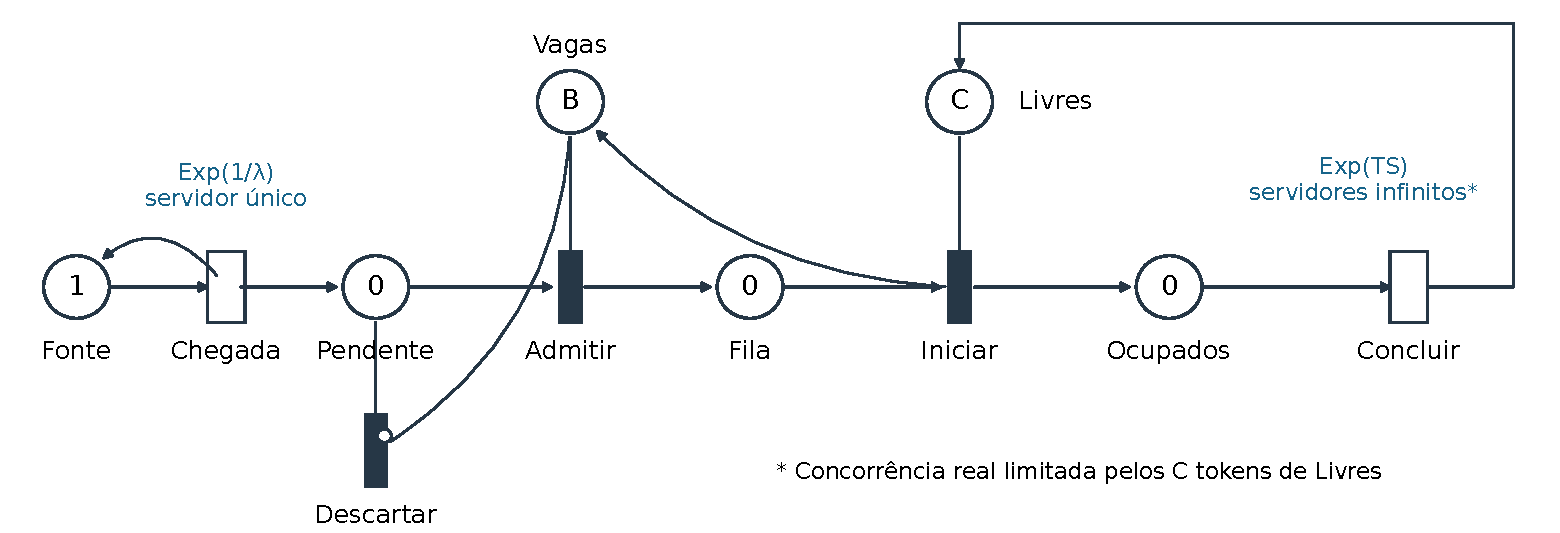
\includegraphics[width=\textwidth]{figuras/modelo_spn.pdf}
\caption{Rede SPN do servidor web avaliada no Jupiter. Círculos representam lugares; barras preenchidas, transições imediatas; retângulos vazados, transições exponenciais. O círculo aberto na ponta do arco de Vagas para Descartar indica inibição.}
\label{fig:spn}
\end{figure*}

\section{Modelagem do sistema}
\subsection{Lugares, marcação e fluxo}
A Figura~\ref{fig:spn} mostra a rede implementada. As chegadas seguem um processo de Poisson de taxa $\lambda$, e o tempo de serviço é exponencial com média $TS=0{,}1$ s. Isso significa que cada servidor consegue atender, em média, dez requisições por segundo. Esses valores foram escolhidos para o exercício e não vieram de medições de uma aplicação real. Na rede, cada token é uma marca que representa uma requisição ou um recurso disponível, conforme o lugar em que está.

\begin{table}[h]
\centering
\caption{Lugares e marcação inicial da rede.}
\label{tab:lugares}
\begin{tabular}{lll}
\toprule
Lugar & Inicial & Significado\\
\midrule
Fonte & 1 & Habilita chegadas externas\\
Pendente & 0 & Requisição em admissão\\
Vagas & $B$ & Vagas livres na fila\\
Fila & 0 & Requisições aguardando\\
Livres & $C$ & Servidores disponíveis\\
Ocupados & 0 & Requisições em serviço\\
\bottomrule
\end{tabular}
\end{table}

Chegada consome e devolve o token de Fonte, além de produzir um token em Pendente. Ela utiliza política de servidor único e atraso médio $1/\lambda$. Isso mantém a demanda externa ativa mesmo quando a fila está cheia. Admitir consome Pendente e Vagas e produz Fila. Descartar consome Pendente, mas um arco inibidor com peso 1 vindo de Vagas só permite seu disparo quando não há vaga disponível.

Iniciar consome um token de Fila e outro de Livres, produzindo Ocupados e devolvendo uma vaga. Essa transição imediata tem prioridade 2; as demais imediatas possuem prioridade 1 e peso 1. Concluir consome Ocupados e devolve Livres. Sua política é de servidores infinitos, com média $TS$. Apesar do nome dessa política, o número de atendimentos ao mesmo tempo continua limitado aos $C$ servidores. Uma requisição só começa quando há um token em Livres.

Os arcos têm peso unitário. As decisões e o início do serviço não acrescentam atraso artificial. Não se acumulam tokens de requisições concluídas: a saída é representada pelo disparo de Concluir. Dessa forma, a rede continua limitada. A soma das requisições na Fila com as vagas livres é sempre $B$. Da mesma forma, a soma dos servidores livres com os ocupados é sempre $C$. Essas relações ajudam a conferir se a rede mantém os limites definidos.

\subsection{Métricas de desempenho}
Foram usadas seis medidas: vazão (TP), tempo médio de resposta (MRT), tempo médio de espera (MQT), utilização dos servidores (U), probabilidade de descarte (DP) e tempo médio de processamento (MPT). A resposta inclui espera e processamento. Nas fórmulas, $\mq$ é a quantidade média de requisições na fila e $\mb$ é a quantidade média em atendimento. As expressões cadastradas no Jupiter são:
\begin{align}
TP &= \mb/TS \quad [\text{requisições/s}],\label{eq:tp}\\
MRT &= (\mq+\mb)/TP \quad [\text{s}],\label{eq:mrt}\\
MQT &= \mq/TP \quad [\text{s}],\label{eq:mqt}\\
U &= 100\,\mb/C \quad [\%],\label{eq:u}\\
DP &= 100\,P(\#Vagas=0) \quad [\%],\label{eq:dp}\\
MPT &= \mb/TP \quad [\text{s}].\label{eq:mpt}
\end{align}

Na expressão de DP, $P(\#Vagas=0)$ é a probabilidade de não haver vaga livre na fila. O símbolo $\#$ indica a quantidade de tokens no lugar. As equações de tempo usam a Lei de Little \cite{little}, com a vazão das requisições aceitas. Usar diretamente a taxa externa em um sistema com perdas subestimaria esses tempos. No arquivo do modelo, as divisões têm uma condição que retorna zero se $\mb=0$. Neste estudo, as taxas positivas permitem calcular as métricas em todos os cenários.

Para as chegadas de Poisson deste modelo, a propriedade PASTA \cite{wolff} permite usar a parcela do tempo em que a fila está cheia para estimar a parcela de chegadas descartadas. Por isso, DP foi calculado pela probabilidade de não haver vaga. Em média, a vazão deve corresponder à taxa de chegada descontando as requisições recusadas.

MRT e MQT descrevem requisições aceitas e posteriormente concluídas. O descarte não é contado como atendimento rápido. MPT é igual a $TS$ pela forma como a fórmula foi definida, então esse resultado sozinho não confirma se o tempo de serviço escolhido representa uma aplicação real. O modelo calcula médias e não acompanha a ordem de atendimento de cada cliente nem os maiores tempos de resposta.

\begin{table*}[!t]
\centering
\caption{Parâmetros e resultados consolidados dos 14 cenários principais. $\lambda$ e TP em requisições/s; tempos em segundos; U e DP em percentual. Em todas as linhas, $TS=MPT=0{,}1$ s. Os valores vêm das tabelas do Jupiter, com quatro casas decimais na origem.}
\label{tab:consolidada}
\begin{tabular}{lrrrrrrrr}
\toprule
Cenário & $\lambda$ & $C$ & $B$ & TP & MRT & MQT & U & DP\\
\midrule
E1-1 & 5 & 2 & 10 & 4,9963 & 0,1068 & 0,0068 & 24,9815 & 0,0000\\
E1-2 & 10 & 2 & 10 & 9,9988 & 0,1332 & 0,0332 & 49,9942 & 0,0163\\
E1-3 & 15 & 2 & 10 & 14,8954 & 0,2081 & 0,1081 & 74,4768 & 0,9533\\
E1-4 & 20 & 2 & 10 & 18,3984 & 0,3388 & 0,2388 & 91,9919 & 7,9789\\
E1-5 & 25 & 2 & 10 & 19,6685 & 0,4475 & 0,3475 & 98,3425 & 21,1799\\
\midrule
E2-1 & 20 & 1 & 10 & 9,9976 & 1,0005 & 0,9005 & 99,9764 & 49,9939\\
E2-2 & 20 & 2 & 10 & 18,3984 & 0,3388 & 0,2388 & 91,9919 & 7,9789\\
E2-3 & 20 & 3 & 10 & 19,9228 & 0,1411 & 0,0411 & 66,4094 & 0,2555\\
\midrule
E3-1 & 20 & 2 & 2 & 15,5498 & 0,1429 & 0,0429 & 77,7491 & 22,2648\\
E3-2 & 20 & 2 & 10 & 18,3984 & 0,3388 & 0,2388 & 91,9919 & 7,9789\\
E3-3 & 20 & 2 & 18 & 19,0225 & 0,5379 & 0,4379 & 95,1126 & 4,8200\\
\midrule
E4-1 & 15 & 2 & 10 & 14,8954 & 0,2081 & 0,1081 & 74,4768 & 0,9533\\
E4-2 & 25 & 2 & 10 & 19,6685 & 0,4475 & 0,3475 & 98,3425 & 21,1799\\
E4-3 & 25 & 4 & 10 & 25,0140 & 0,1205 & 0,0205 & 62,5350 & 0,1097\\
\bottomrule
\end{tabular}
\end{table*}

\section{Simulações e resultados}
\subsection{Planejamento experimental}
A referência foi definida com $\lambda=20$ requisições/s, $C=2$, $B=10$ e $TS=0{,}1$ s. A demanda coincide com a capacidade nominal de atendimento, $C/TS=20$ requisições/s. Essa escolha permite observar o que acontece quando a demanda alcança a capacidade média dos servidores e comparar formas de melhorar o atendimento. A carga foi escolhida para o exercício.

E1 usa cinco níveis de demanda, de 5 a 25 requisições/s, com incremento de 5. E2 mantém a demanda em 20 e testa um, dois e três servidores. E3 mantém essa mesma demanda e dois servidores, alterando a fila para 2, 10 e 18 vagas. Os limites foram escolhidos para representar uma fila curta, a referência e uma ampliação com o mesmo incremento de oito vagas.

E4 compara três situações: demanda de 15 com dois servidores, demanda de 25 mantendo dois servidores e demanda de 25 com quatro servidores. A fila permanece com dez vagas. A interface testou todas as combinações entre as demandas de 15 e 25 e as quantidades de dois e quatro servidores. O caso adicional de 15 com quatro servidores foi mantido nos dados para comparação. Esse caso não substitui os três casos principais da Tabela~\ref{tab:consolidada}.

\subsection{Procedimento e conferência}
Foi utilizada a opção \textit{Stationary Simulation} do Jupiter 1.17.0 para estudar o comportamento do sistema após o período inicial. Essa escolha permite comparar o desempenho mantido ao longo do tempo. Cada configuração foi avaliada por 5.000 s, com aquecimento de 500 s, 30 repetições e semente 707. O aquecimento descarta o início da execução, quando a fila ainda está vazia. A semente permite repetir a sequência de números aleatórios usada na simulação. O nível de confiança foi configurado em 95\%, com erro relativo alvo de 2\%. O limite de eventos foi 1.000.000, o paralelismo foi 4 e o limite de tempo da execução foi 60 s. Os valores configurados estão descritos nos arquivos do projeto.

Como a quantidade de repetições foi fixada em 30, o erro alvo de 2\% não garante essa precisão para todas as medidas. Isso merece atenção principalmente quando o descarte é raro. Um zero na tabela pode ser resultado do arredondamento ou de não terem ocorrido descartes na amostra. Também não é possível afirmar, apenas pelo tempo de uma execução, que o sistema já chegou a um comportamento estável.

Como conferência, o cenário de referência foi reavaliado com horizonte de 10.000 s. O MRT passou de 0,338783 para 0,339137 s, diferença de aproximadamente 0,10\%. Os intervalos de 95\% foram, respectivamente, [0,3371; 0,3404] e [0,3382; 0,3400] s. A vazão ficou em 18,398385 e 18,398083 requisições/s. A pequena mudança sugere que aumentar o tempo da simulação teve pouco efeito nesse caso, embora isso não garanta a mesma precisão nos outros cenários.

Também foi feita uma conferência separada com um modelo matemático de filas. Ele considera as mesmas hipóteses: chegadas de Poisson, serviço exponencial, vários servidores e capacidade limitada. A maior diferença no MRT dos 14 cenários foi inferior a 0,5\%. Esse cálculo foi usado apenas para conferir a coerência dos valores. Os dados da tabela e dos gráficos continuam sendo os resultados das simulações no Jupiter.

Os arquivos CSV mantêm as quatro casas decimais mostradas nas tabelas de cenários. O arquivo exportado do caso de referência também contém intervalos de confiança, que indicam a incerteza das médias estimadas. Para os demais casos, foram usados os valores disponíveis, sem acrescentar intervalos que a tabela não forneceu.

\begin{figure*}[!t]
\centering
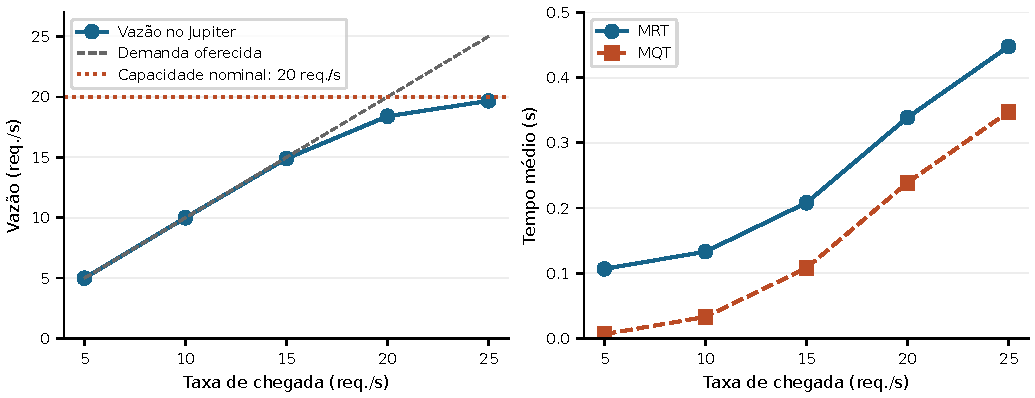
\includegraphics[width=\textwidth]{figuras/e1_demanda.pdf}
\caption{E1: efeito da demanda sobre vazão e tempos médios, com $C=2$, $B=10$ e $TS=0{,}1$ s. A linha de demanda mostra quantas requisições chegam por segundo; a vazão mostra quantas são atendidas.}
\label{fig:e1}
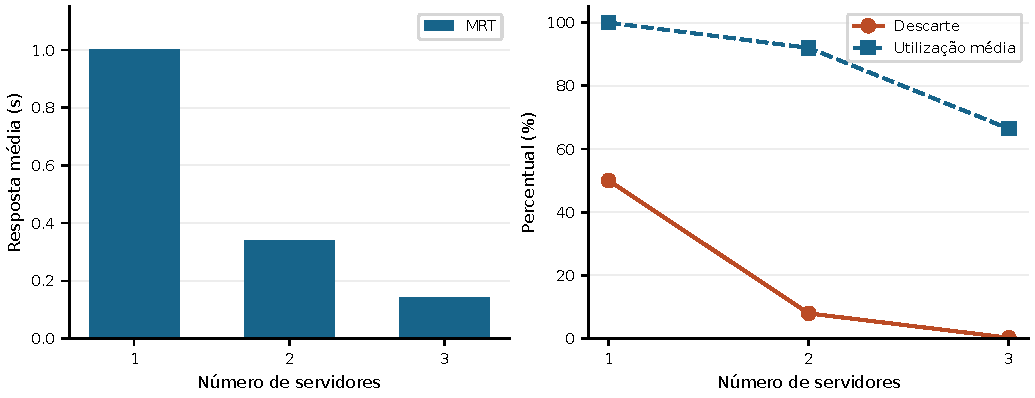
\includegraphics[width=\textwidth]{figuras/e2_servidores.pdf}
\caption{E2: efeito do número de servidores sobre resposta, descarte e utilização. Demanda fixa em 20 requisições/s e fila de dez vagas.}
\label{fig:e2}
\end{figure*}

\subsection{E1: efeito da demanda}
A Figura~\ref{fig:e1} mostra que a vazão acompanha a demanda enquanto existe folga de processamento. Com cinco requisições/s, a utilização média é de aproximadamente 25\% e o MRT fica próximo do próprio tempo de serviço, em 0,1068 s. Ao chegar a 15 requisições/s, a utilização sobe para 74,48\% e a espera média já alcança 0,1081 s, valor ligeiramente superior ao tempo gasto em processamento.

Na taxa de 20 requisições/s, a vazão é de 18,3984, e não de 20. Embora a capacidade nominal também seja 20, as chegadas e os serviços variam aleatoriamente. O sistema alterna momentos com recursos livres e momentos com fila cheia. Com capacidade finita, a igualdade entre demanda e capacidade nominal não elimina descartes.

Ao aumentar a demanda de 20 para 25, a utilização vai de 91,99\% para 98,34\%, mas a vazão cresce apenas cerca de 6,9\%. O descarte passa de 7,98\% para 21,18\%. A resposta média aumenta para 0,4475 s, sendo 0,3475 s de espera. Portanto, o ganho de vazão vem acompanhado de piora no atendimento e de maior rejeição de requisições.

\subsection{E2: efeito dos servidores}
Com um servidor, a demanda de 20 requisições/s corresponde ao dobro de sua taxa média de serviço. O recurso fica praticamente sempre ocupado, a vazão se aproxima de dez e cerca de metade das chegadas é descartada. O MRT de 1,0005 s é formado principalmente pela espera de 0,9005 s. Esse caso evidencia o gargalo no atendimento.

Dois servidores melhoram a vazão, mas ainda deixam o sistema operando próximo de sua capacidade. Com três, o MRT cai para 0,1411 s e o descarte para 0,2555\%. A redução do MRT em relação a dois servidores é de aproximadamente 58,4\%. A utilização cai para 66,41\%, o que representa margem para absorver variações, e não necessariamente desperdício. Entre as três alternativas avaliadas para a demanda de 20, essa configuração apresenta o melhor equilíbrio entre recursos e os indicadores considerados.

\begin{figure*}[!t]
\centering
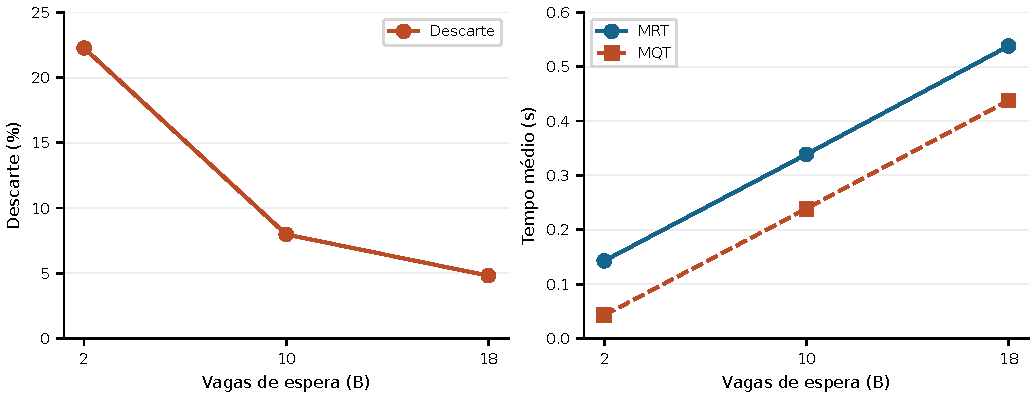
\includegraphics[width=\textwidth]{figuras/e3_fila.pdf}
\caption{E3: efeito do limite de espera, mantendo 20 requisições/s e dois servidores. Uma fila maior reduz descartes, mas aumenta a permanência das requisições aceitas.}
\label{fig:e3}
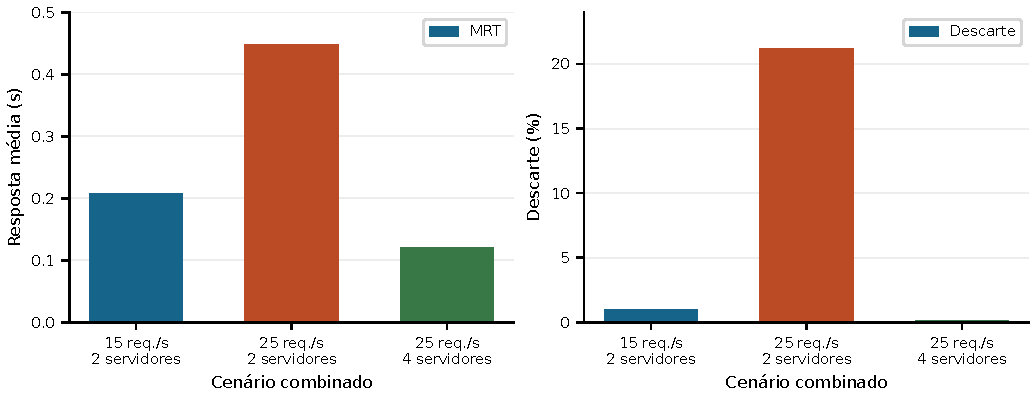
\includegraphics[width=\textwidth]{figuras/e4_combinados.pdf}
\caption{E4: três cenários principais de demanda e recursos. Em todos, $B=10$ e $TS=0{,}1$ s. Os valores são as médias estimadas nas simulações do Jupiter.}
\label{fig:e4}
\end{figure*}

\subsection{E3: efeito da fila}
Na Figura~\ref{fig:e3}, a fila de duas vagas apresenta descarte de 22,2648\% e MRT de 0,1429 s. O tempo menor não significa que todas as requisições recebem atendimento melhor: uma parcela maior sequer é aceita. Esse resultado precisa ser interpretado junto com a vazão de 15,5498 requisições/s.

Com dez vagas, o descarte diminui para 7,9789\% e a vazão sobe para 18,3984. Entretanto, o MRT cresce para 0,3388 s. A fila absorve mais requisições em períodos de acúmulo, mas os dois servidores continuam processando com a mesma taxa. Portanto, aumentar o espaço de espera não resolve a limitação do atendimento.

Ao ampliar de dez para dezoito vagas, a vazão cresce apenas cerca de 3,4\%, chegando a 19,0225 requisições/s. Já o MRT cresce aproximadamente 58,8\%, para 0,5379 s. A fila média passa de 4,3935 para 8,3306 requisições. A ampliação reduz perdas para 4,82\%, mas mantém uma espera elevada. Nesse conjunto, o custo aparece como maior atraso, mesmo sem calcular um custo financeiro.

\subsection{E4: demanda e recursos juntos}
O primeiro caso da Figura~\ref{fig:e4} apresenta 15 requisições/s com dois servidores: MRT de 0,2081 s e descarte de 0,9533\%. Ao aumentar a demanda para 25 e manter os recursos, o descarte sobe para 21,1799\% e a resposta para 0,4475 s. Essa comparação mostra o risco de conservar uma configuração quando a carga muda.

Com quatro servidores na demanda de 25, o MRT cai para 0,1205 s e o descarte para 0,1097\%. A utilização média é de 62,5350\%. A redução do MRT em relação ao caso sobrecarregado é de aproximadamente 73,1\%. A vazão estimada de 25,0140 fica ligeiramente acima da taxa externa de 25 porque a vazão foi estimada a partir da ocupação média dos servidores. A diferença é inferior a 0,2\% e faz parte da incerteza da simulação. Ela não significa que o sistema gerou requisições a mais.

\subsection{Gargalo e recomendação de dimensionamento}
Os experimentos indicam que a capacidade de processamento é o principal gargalo do sistema representado. Em E1, aumentar a demanda aproxima os servidores da ocupação total e amplia a fila. Em E3, aumentar somente as vagas melhora a aceitação, porém mantém a taxa de atendimento. E2 mostra que ampliar os recursos de processamento reduz tanto a espera quanto o descarte.

Para tornar a recomendação objetiva, foram adotados dois critérios para esta comparação: MRT abaixo de 0,25 s e descarte abaixo de 1\%, procurando usar a menor quantidade de servidores entre as alternativas avaliadas para a mesma demanda. Esses limites foram escolhidos para a comparação deste trabalho; não são uma exigência do enunciado nem metas fornecidas por uma aplicação real.

Na demanda de 20 requisições/s, um e dois servidores não atendem a esses critérios. Três servidores, com dez vagas, apresentam MRT de 0,1411 s e descarte estimado de 0,2555\%. Assim, recomenda-se essa configuração entre as opções de E2. O ganho em relação à referência é mais interessante do que ampliar a fila para dezoito vagas, pois essa ampliação ainda apresenta descarte de 4,82\% e resposta de 0,5379 s.

Na demanda de 25 requisições/s, quatro servidores com dez vagas atendem aos critérios considerando as médias obtidas. Essa é a opção recomendada entre as configurações testadas para essa carga. O trabalho não avaliou três servidores nessa taxa; portanto, não é possível afirmar que quatro seja a menor quantidade necessária. Seria preciso testar também três servidores e avaliar a incerteza dos resultados antes de aceitar valores muito próximos das metas.

O caso de 15 requisições/s com dois servidores fica próximo da meta de 1\% de descarte. Mesmo com média de 0,9533\%, seria inadequado tratá-lo como garantia de cumprimento do limite. Para uma aplicação real, seria necessário deixar uma margem, fazer mais repetições e medir a demanda. Não foi calculado o custo financeiro de cada configuração. A quantidade de servidores foi usada apenas para comparar quanto recurso cada opção exige.

\subsection{Limitações do estudo}
O modelo supõe chegadas independentes e tempos exponenciais de serviço. Na prática, muitas requisições podem chegar juntas, ter tamanhos diferentes e levar tempos bastante diferentes para serem processadas. Não foram representados atrasos de rede, comunicação entre máquinas, disco, banco de dados, falhas ou concorrência interna de um servidor. Logo, não se pode usar diretamente estes números para contratar infraestrutura de uma aplicação específica.

A avaliação usa médias, que não mostram sozinhas o que acontece com as requisições mais demoradas. A conferência matemática ajuda a verificar se os cálculos estão coerentes, mas não confirma se as hipóteses representam uma aplicação real. Os gráficos também não mostram a incerteza de cada média. Os intervalos disponíveis para o caso de referência foram discutidos na metodologia e não devem ser usados como se valessem para todos os cenários.

\section{Conclusão}
O modelo SPN construído no Jupiter permitiu comparar os efeitos da demanda, dos servidores e da capacidade da fila em um serviço web simplificado. A demanda maior aumentou a ocupação dos recursos, os tempos de espera e os descartes. Aumentar somente a fila reduziu perdas, mas fez as requisições aceitas esperarem mais. Já o aumento do número de servidores trouxe melhora simultânea desses indicadores nos casos estudados.

Entre as opções avaliadas, três servidores com dez vagas oferecem uma alternativa adequada para 20 requisições/s. Para a carga de 25, a opção de quatro servidores com dez vagas apresentou o melhor resultado entre as configurações testadas. Como continuidade, seria útil medir uma aplicação real, ajustar os tempos de chegada e de serviço e considerar os custos e as requisições mais demoradas. Outra possibilidade seria estudar o aumento automático da quantidade de servidores, levando em conta o tempo necessário para ativá-los.

\noindent\textbf{Materiais do trabalho:} modelo, configurações, dados e códigos disponíveis no repositório \url{https://github.com/SamuelTorres51/SD-Jupiter-07}.\par
\noindent\textbf{Apresentação em vídeo:} pendente de gravação e publicação pelo autor. O link deverá ser incluído nesta versão antes da entrega no SIGAA.

\begin{thebibliography}{6}
\bibitem{murata} T. Murata, ``Petri nets: Properties, analysis and applications,'' \textit{Proceedings of the IEEE}, vol. 77, no. 4, pp. 541--580, 1989, doi: \href{https://doi.org/10.1109/5.24143}{10.1109/5.24143}.
\bibitem{marsan} M. Ajmone Marsan, G. Conte e G. Balbo, ``A class of generalized stochastic Petri nets for the performance evaluation of multiprocessor systems,'' \textit{ACM Transactions on Computer Systems}, vol. 2, no. 2, pp. 93--122, 1984, doi: \href{https://doi.org/10.1145/190.191}{10.1145/190.191}.
\bibitem{macedo} J. Macêdo, V. Carvalho, E. Andrade e F. A. Silva, ``Modelagem e análise da comunicação em VANETs com uso de RSUs,'' em \textit{Workshop em Desempenho de Sistemas Computacionais e de Comunicação}, SBC, 2022, doi: \href{https://doi.org/10.5753/wperformance.2022.223324}{10.5753/wperformance.2022.223324}.
\bibitem{jupiter} Jupiter Analytics, ``Jupiter Wiki: model building, metrics and execution \& analysis.'' Disponível em: \url{https://wiki.jupiteranalytics.com.br/}. Acesso em: 15 nov. 2026.
\bibitem{little} J. D. C. Little, ``A proof for the queuing formula: $L=\lambda W$,'' \textit{Operations Research}, vol. 9, no. 3, pp. 383--387, 1961, doi: \href{https://doi.org/10.1287/opre.9.3.383}{10.1287/opre.9.3.383}.
\bibitem{wolff} R. W. Wolff, ``Poisson arrivals see time averages,'' \textit{Operations Research}, vol. 30, no. 2, pp. 223--231, 1982, doi: \href{https://doi.org/10.1287/opre.30.2.223}{10.1287/opre.30.2.223}.
\end{thebibliography}
\end{document}
